\subsection{Configuración Experimental}

Para realizar todos los ensayos, se utilizó como instrumento de medición un osciloscopio digital doble canal Tektronix TBS1102B de \SI[]{100}{\mega\hertz} de ancho de banda y 2 GS/s, tal como el que se observa en la figura \ref{test_setup}. Para alimentar la tensión y corriente de entrada al convertidor, se utilizó una fuente de laboratorio de corriente continua HP 6010A, visible en la esquina superior derecha de la imagen, con capacidad de hasta \SI[]{200}{\volt}, \SI[]{17}{\ampere} y \SI[]{1000}{\watt}. Finalmente, para simular las condiciones de carga a la salida de la plataforma, se utilizo la carga electrónica variable ITECH I8514B+ que se mencionó en el capítulo \ref{analisis}, presente en la figura debajo de la fuente de laboratorio.\\

\begin{figure}[h]
    \centering
    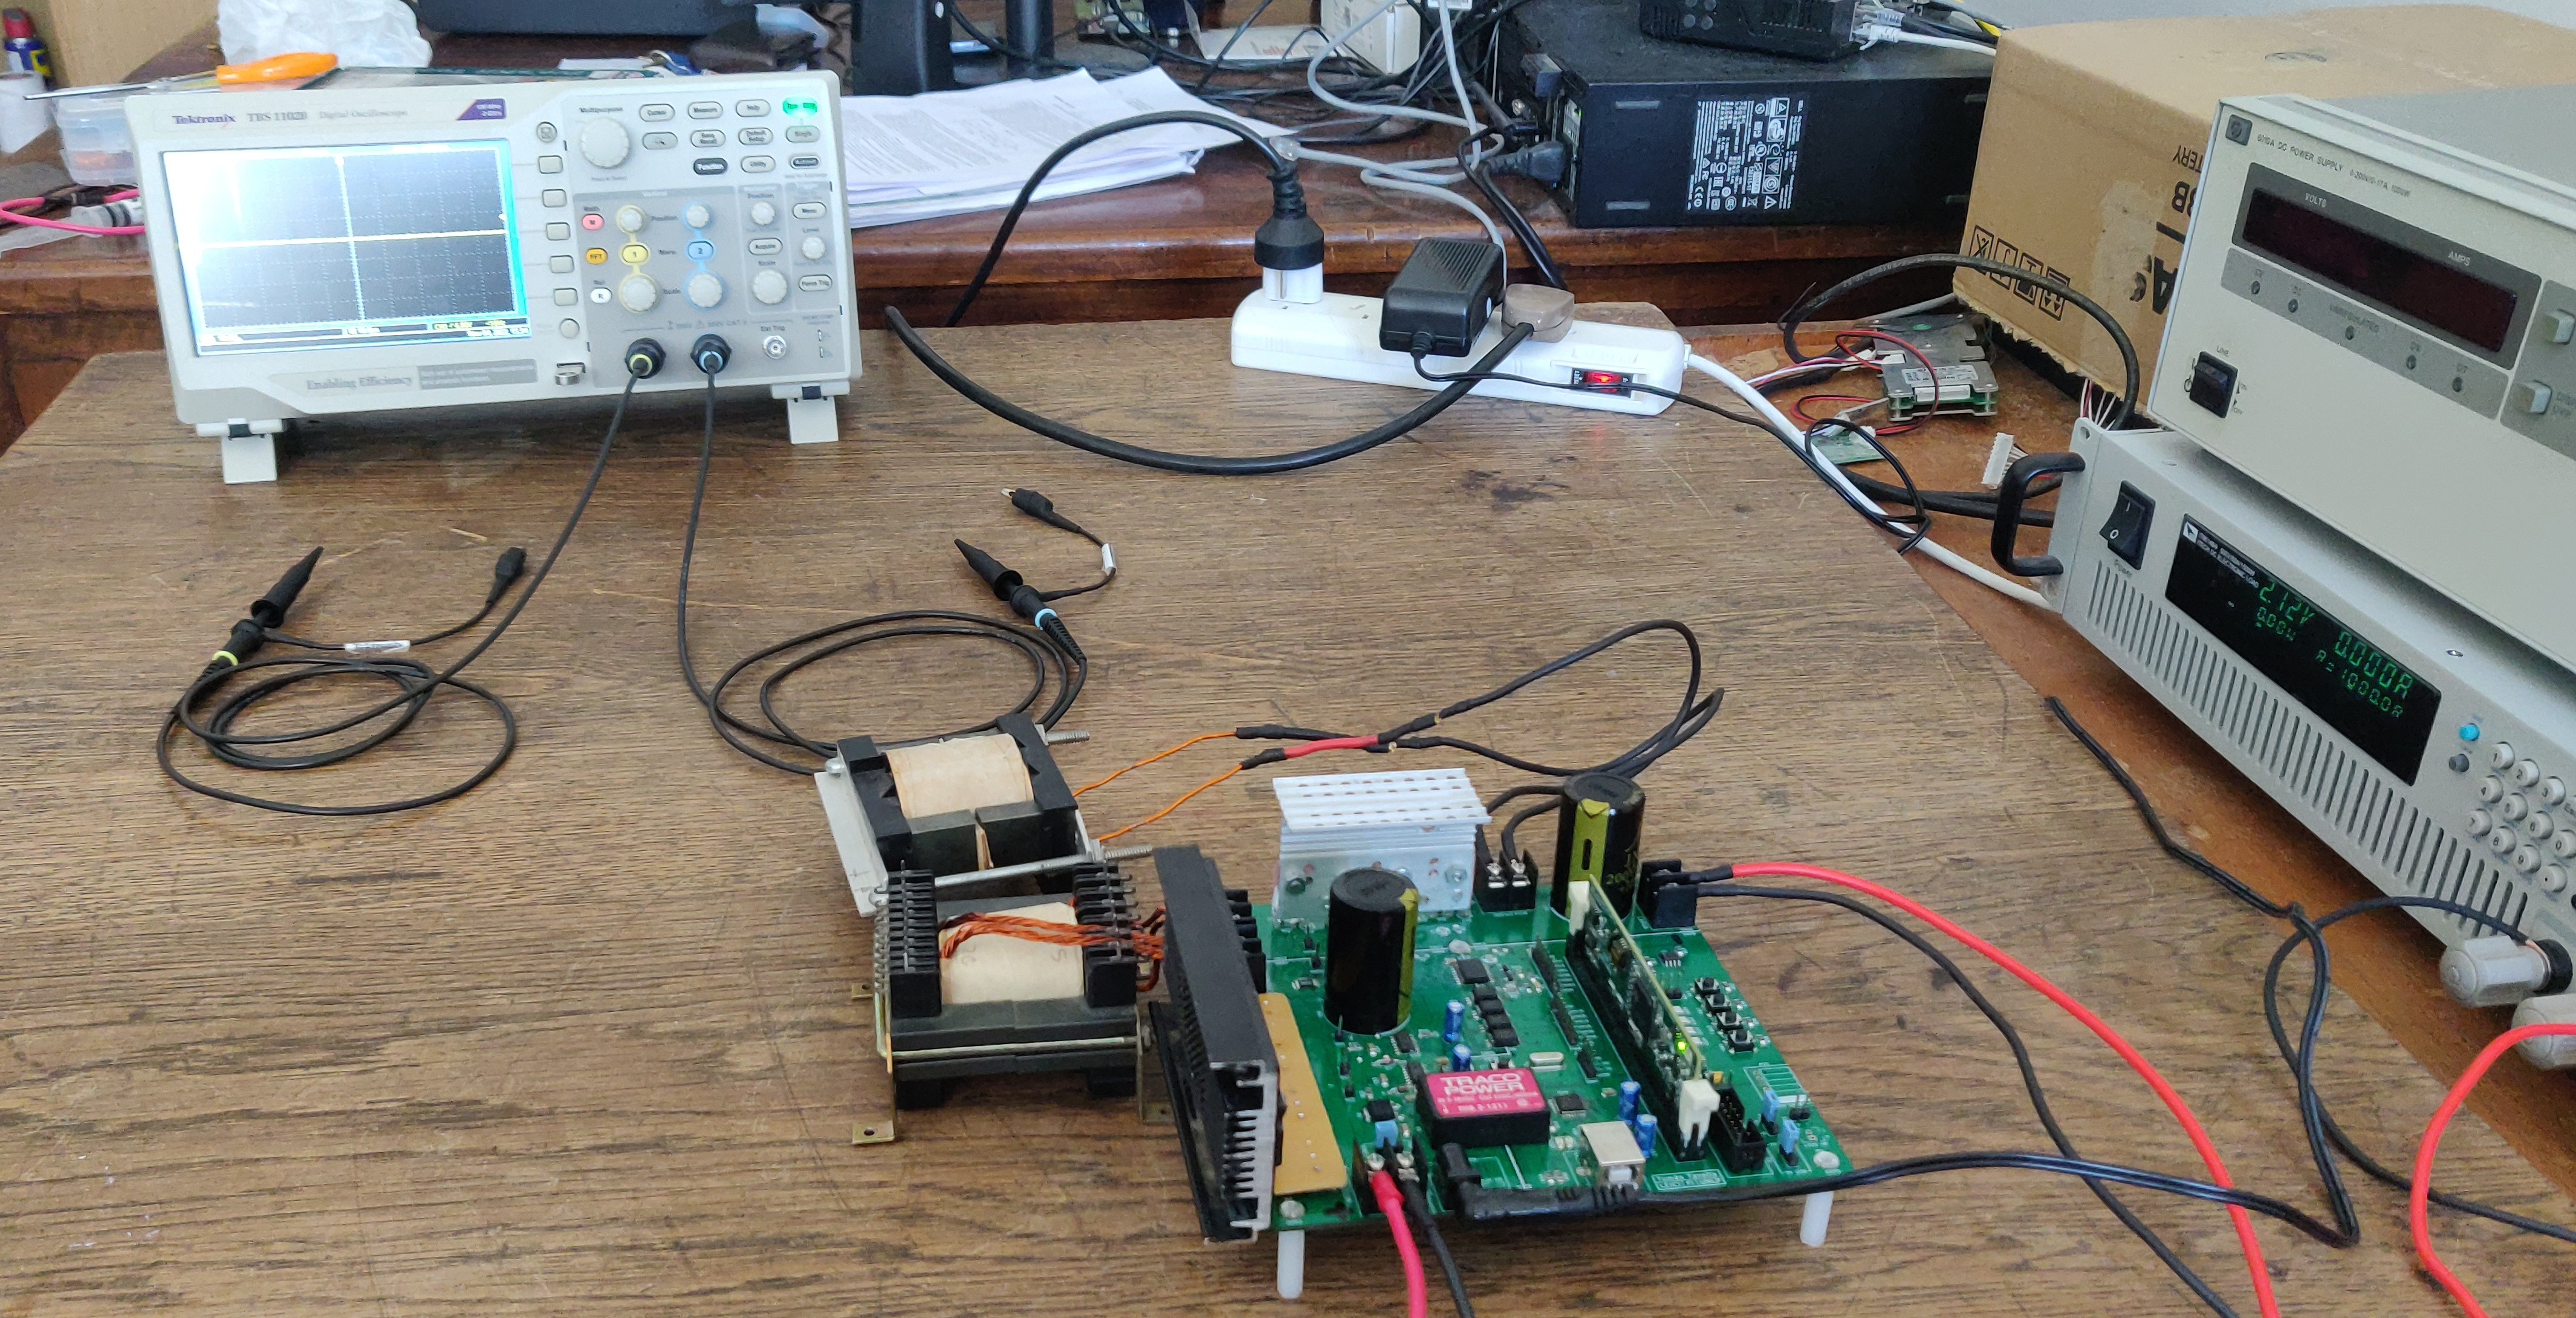
\includegraphics[scale=0.09]{Imagenes/Setup Ensayo.jpg}
    \caption{Setup utilizado para la realización de los ensayos de evaluación del convertidor CC-CC puente completo.}
    \label{test_setup}
\end{figure}

Para poder realizar todas las pruebas, también fue necesaria la programación de un firmware mínimo que pusiera en funcionamiento los módulos ePWM necesarios para generar las señales de comando, que luego son enviadas a los circuitos driver y generan la excitación del puente de MOSFET. Además, se agregó un código que, mediante interrupciones externas, varía el ciclo de trabajo mediante el accionamiento de dos pulsadores, y genera una indicación del mismo utilizando cuatro LEDs.\\

Este firmware se programó en lenguaje C, utilizando el IDE provisto por Texas Instruments, llamado \textit{Code Composer Studio} (CCS), que incluye un compilador, bibliotecas y las herramientas de software necesarias para cargar los programas al controlador. Como la carga y debugging del firmware se realiza a través del puerto JTAG, se utiliza una \textit{docking station} para el controlador, provista por Texas Instruments, que cuenta con la capacidad de emular la funcionalidad de JTAG a través de USB, y actúa como intermediario entre el puerto USB de la computadora y el puerto JTAG de la plataforma.\\ 

\begin{figure}[h]
    \centering
    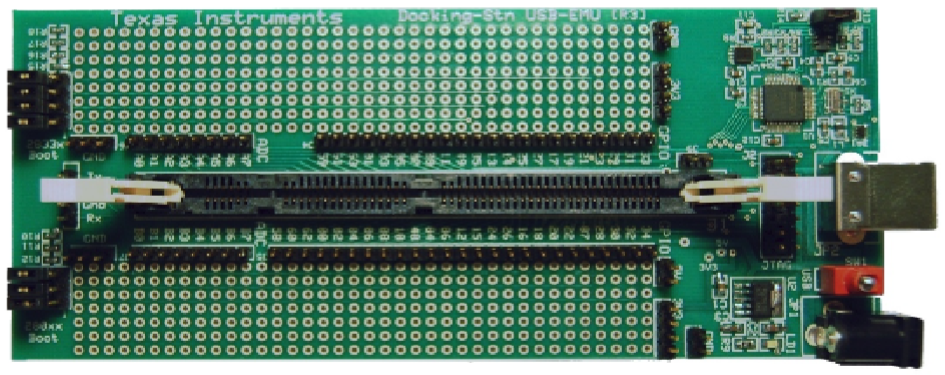
\includegraphics[scale=0.25]{Imagenes/Docking Station.png}
    \caption{Docking station para controlCARD de la serie C2000, con el puerto USB y JTAG a la derecha.}
    \label{docking_station}
\end{figure}